这样做的好处是,热指令都会存在同一个cache line里,可以提高CPU前端数据结构的利用效率,例如I-cache 和 DSB-Cache

\begin{figure}[H]
    \centering
    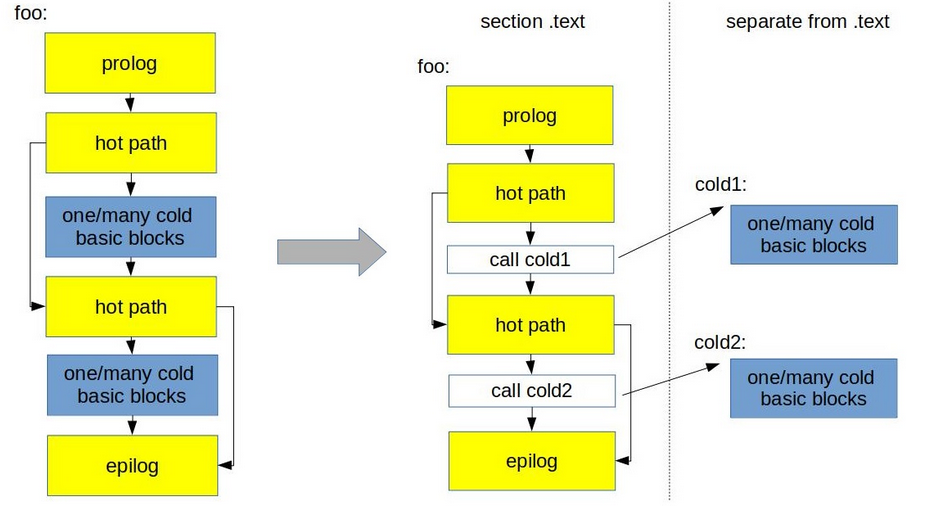
\includegraphics[width=0.53\textwidth]{images/splitting.png}
    \caption{将冷代码过程转换为函数调用}
\end{figure}